\chapter{Sviluppo Front-end con OpenLayers}
\label{cap:chapter4}

In questo capitolo verrà esaminato in dettaglio il funzionamento della libreria di OpenLayers e le ragioni che hanno portato alla sua scelta come strumento principale per l'implementazione delle mappe nell'ambito del progetto. Successivamente, saranno poi esposte le prime implementazioni, ancora prive di un back-end, realizzate dal candidato con questa libreria, ponendo l'attenzione su tutte le problematiche da lui riscontrate fino al raggiungimento di una soluzione.

\section{Introduzione a OpenLayers}

OpenLayers è una libreria open source JavaScript che fornisce strumenti per la visualizzazione di mappe interattive su pagine web. Fornisce grande capacità di astrazione per gli sviluppatori, andando ad incapsulare tutte le funzionalità dei servizi menzionati fino ad ora. 

\subsection{Caratteristiche principali}
Una delle caratteristiche principali di OpenLayers è la sua capacità di offrire un interfaccia grafica di mappe omogenea su diversi tipi di dispositivi e browser. Essa permette, in modo intuitivo e conciso, di accedere a una serie di funzionalità basilari, quali zoom, capacità di trascinare la mappa e interazione con elementi a schermo (come marker o punti).
\\Offre inoltre API ad alto livello che consentono di integrare facilmente diversi tipi di servizi geospaziali nei progetti, come WMS, WMTS, WFS, TMS etc...
Sono supportati anche formati strettamente geospaziali, tra cui GeoJSON, KML, etc... L'accesso a questi dati è possibile sia contattando un server esterno, senza aver bisogno di utilizzare esplicitamente i servizi sopra citati, sia salvando i relativi file direttamente in locale per poi accedervi.
\\Infine, OpenLayers supporta di default alcuni provider di mappe, tra cui: OpenStreetMap, Bing Maps, Google Maps, etc... Ciò non preclude la possibilità di utilizzare altri servizi di mappe esterni.

\subsection{Architettura di OpenLayers}

Il lavoro di tirocinio è iniziato con lo studio e l'utilizzo di tale libreria, partendo dalla creazione di una piccola applicazione esterna al progetto aziendale. Questa scelta è stata fatta per acquisire una comprensione approfondita del suo funzionamento, in modo poi da poterla poi confrontare con la versione già iniziata dall'azienda. In questo procedimento, il candidato ha deciso di privare tale applicazione del framework Angular e di librerie di terze parti, così da semplificare il suo utilizzo.
\\Lo studio da parte del candidato è quindi cominciato con la consultazione della documentazione ufficiale \cite{DocumentazioneOpenLayersBase}, la quale riporta i quattro componenti principali su cui si basa OpenLayers:
\begin{itemize}
    \item ol/Map: è il core della libreria, rappresenta la mappa stessa e fornisce funzionalità di base come la gestione dei layer, degli eventi e delle view.
    \item ol/View: si occupa di gestire la View (la vista) della mappa, controlla la proiezione e il livello di zoom della mappa. La vista determina cosa viene mostrato sulla mappa e in quale modo.
    \item ol/source: fornisce classi per definire le fonti di dati per i layer, ad esempio fonti WMS, WFS, GeoJSON, ecc.
    \item ol/layer: si occupa della creazione dei layer sulla mappa
\end{itemize}
Essendo una libreria open source, il suo codice è interamente disponibile su GitHub \cite{GithubOpenLayers}, completo di documentazione ufficiale in cui vengono spiegati nel dettaglio tutti gli altri suoi componenti.
\\Per comprendere meglio il suo utilizzo, qui di seguito viene riportata una parte del codice semplificata, realizzata dal tirocinante, per l'applicazione esterna menzionata precedentemente:
\lstinputlisting[language=html, caption={Esempio di implementazione OpenLayers - HTML}]{listings/Capitolo3/index.html}
\lstinputlisting[caption={Esempio di implementazione OpenLayers - JavaScript}, language=Java]{listings/Capitolo3/main.js}
Nell'esempio qui riportato, il codice istanzia un oggetto mappa utilizzando la classe \verb|Map| fornita dalla libreria. Questa mappa è indirizzata a un elemento HTML specifico identificato dall'id 'map';  questo è l'elemento HTML in cui la mappa verrà poi visualizzata. All'interno dell'oggetto mappa, viene definita una \verb|View| che imposta la telecamera al centro con uno livello di zoom iniziale. Infine, viene creato un singolo layer che mostra la mappa di base fornita da OpenStreetMap, utilizzando la classe \verb|OSM()|.

\subsection{Perché OpenLayers}

Tale libreria è stata scelta rispetto alle altre concorrenti, in quanto offre internamente un supporto già integrato ai protocolli OGC sopra menzionati, essenziali in questo contesto di sviluppo, poiché la maggioranza della mappe da integrare all'interno dell'applicazione erano fornite tramite questi ultimi.
\\Con l'utilizzo di questa libreria, infatti, la comunicazione ai servizi OGC esterni risulta essere più semplice, in quanto non è necessario eseguire manualmente tutte le richieste imposte dallo Standard, e, successivamente, eseguire il parsing sul contenuto delle risposte in formato XML. OpenLayers fornisce, a più livelli, delle classi che si occupano di eseguire queste operazioni al posto nostro, esponendo allo sviluppatore solo il minimo necessario per eseguire correttamente la richiesta.
\\Per esempio, nel caso dell'implementazione del protocollo WMS, se il layer è noto, non sarà necessario eseguire una richiesta di GetCapabilities e successivamente GetMap: basterà istanziare la classe ImageWMS, la quale, una volta passati i parametri corretti, eseguirà automaticamente le operazioni necessarie al fine di ricevere l'immagine della mappa corretta. Qui sotto viene riportato un esempio di implementazione della classe ImageWMS, reperibile anche dalla documentazione di OpenLayers \cite{DocumentazioneOpenLayersWMS}.
\lstinputlisting[language=Java, caption={Esempio di ImageWMS con OpenLayers}]{listings/Capitolo3/openLayersWMS.js}
Come si può vedere dall'implementazione, è sufficiente istanziare la classe ImageWMS passandogli come argomento soltanto l'URL e il layer che si vuole visualizzare. Il campo \verb|serverType| è un argomento facoltativo che serve a specificare quale tipo di server di mappe si sta andando a contattare, ed è utile ad OpenLayers per modificare il modo in cui internamente esegue le richieste. OpenLayers, dopo aver eseguito la richiesta di GetMap, si occuperà anche di mostrare a schermo l'immagine della mappa.
\\Tale esempio richiede ovviamente che il nome del layer sia noto. Nel caso in cui il client non conosca la lista di layer disponibili, sarà comunque necessario eseguire una richiesta di GetCapabilities.
\\Anche in questo caso, OpenLayers si occupa di eseguire la richiesta e di effettuare il parsing in automatico sul contenuto dell'XML, senza dover creare una struttura dati apposita per manipolare i dati ricevuti da essa.
\lstinputlisting[language=Java, caption={Esempio di GetCapabilities per WMS}]{listings/Capitolo3/openLayerWMSCapabilities.js}
\\Inoltre, la libreria dispone di un supporto integrato per il formato GeoJSON, rendendola ideale per le prime implementazioni di mappe, in cui il back-end non è ancora stato sviluppato e c'è bisogno di iniziare a testare le mappe all'interno dell'applicazione. Oltre a ciò, OpenLayers supporta anche l'aggiunta di plugin di terze parti per estendere le sue funzionalità; la sua principale raccolta è disponibile sul loro sito \cite{DocumentazioneOpenLayersPlugin}{}.
\\Infine, la libreria può essere facilmente installata all'interno del progetto tramite l'utilizzo di un gestore di pacchetti come npm o yarn (\texttt{\textdollar\ npm install ol}).

\subsection{Base di partenza}

Il candidato, infine, ha confrontato il suo lavoro con quello già presente all'interno del progetto, così da comprendere meglio le differenze principali fra le due implementazioni e capire quali funzionalità fossero già state realizzate dall'azienda.
\\La versione aziendale aveva una struttura di base simile a quella sviluppata dal tirocinante, utilizzando gli elementi principali di OpenLayers citati sopra. Era stato anche implementato un meccanismo per gestire la sovrapposizione multipla di layer e una funzione di base per la visualizzazione dei marker, la quale sarebbe stata poi utilizzata per mostrare i ponti d'Italia. La parte principale che risultava totalmente assente era il supporto relativo alle carte geografiche, necessarie per valutare la sicurezza di un ponte. La maggior parte di queste mappe erano principalmente fornite da server geografici esterni, i quali, tramite l'uso di protocolli OGC, restituivano i dati delle mappe interessate. Il resto delle mappe erano invece da scaricare in locale, esposte nei formati Shapefile e GeoJSON.
\\Quindi, il compito iniziale del tirocinante è stato quello di sviluppare un sistema in grado di contattare i servizi OGC esterni, supportare i principali formati come Shapefile e GeoJSON e infine implementare un sistema che consentisse di fornire le mappe locali su un servizio esterno, riducendo così la necessità di conservarle localmente all'interno del progetto.
\medskip  
\\La differenza più sostanziosa rispetto all'implementazione aziendale era che, essendo realizzata in Angular, era stato fatto ampio uso dei componenti, permettendo così di esportare facilmente il componente della mappa e di importarlo più volte in pagine web differenti dell'applicazione. Inizialmente, infatti, tale componente era situato all'interno della pagina web dell'Ui-Kit, ovvero una pagina che, a scopo dimostrativo, conteneva tutti i componenti grafici che sarebbero stati poi utilizzati all'interno dell'applicazione.
\begin{figure}[htbp]
    \centering
    \includegraphics[width=1\textwidth]{Tesi/images/Capitolo4/MapComponent.jpg}
    \caption{Il componente Angular delle mappe nell'Ui-Kit}
    \label{fig:MapComponent}
\end{figure}
\\L'uso dell'Ui-Kit è una pratica comune, specialmente nel contesto di applicazioni Enterprise, in quanto permette agli sviluppatori di poter realizzare tutti i componenti indipendentemente dalla pagina web in cui verranno poi collocati. In questo modo è possibile sia mantenere una coerenza visiva fra tutti i componenti dell'applicazione, aiutando così gli sviluppatori front-end a realizzare un'interfaccia uniforme e coincisa, sia come strumento di presentazione del design ai potenziali clienti, così da fornire loro un'anteprima dell'aspetto e delle funzionalità dell'applicazione.
\\Ovviamente l'uso dell'Ui-Kit è reso possibile grazie ai framework JavaScript come Angular, la cui architettura modulare rende possibile l'esportazione dei componenti creati in altre pagine web dell'applicazione. Ad esempio, quando uno sviluppatore crea un componente nell'Ui-Kit, può facilmente importarlo e utilizzarlo all'interno delle varie pagine del sito, senza doverlo ricreare da zero ogni volta. Senza Angular, questa operazione sarebbe molto più laboriosa, dovendo riscrivere più volte lo stesso codice, e quindi non risulterebbe più conveniente. La prima parte di tirocinio si è quindi dedicata al continuo e all'estensione del componente Angular delle mappe, andando ad implementare le funzionalità precedentemente illustrate.

\subsection*{Censimento delle Mappe}

\\Dopo questa fase di apprendimento iniziale, il candidato ha collaborato con l'azienda per identificare le fonti da cui raccogliere le mappe necessarie, censendole in un documento dettagliato. Questo processo ha permesso di avere una panoramica completa delle risorse geospaziali disponibili e di comprendere come organizzarle e utilizzarle nel contesto del tirocinio. Le mappe utilizzate all'interno del progetto provenivano principalmente da tre fonti:
\begin{itemize}
    \item \textit{Geoportale Nazionale}, un portale gestito dal Ministero dell'Ambiente e della Sicurezza Energetica che contiene dati geospaziali forniti tramite protocollo OGC, quali WMS e WFS. É possibile reperire le mappe utilizzate dal loro sito \cite{GeoPortaleNazionale}.
    \item \textit{IdroGEO}, una piattaforma gestita da ISPRA (Istituto Superiore per la Protezione della Ricerca Ambientale), che permette agli utenti di accedere e di scaricare dati di mappe, in formato Shapefile o GeoJSON, relativi al rischio idrogeologico in Italia. Precisamente fornisce informazioni sull'Inventario dei Fenomeni Franosi in Italia (IFFI) e sulle mappe nazionali di pericolosità da frane e alluvioni e sugli indicatori di rischio associati.
    \item \textit{GeoCart}, un'azienda italiana specializzata nella produzione e distribuzione di mappe e prodotti cartografici \cite{GeoCart}. Anche in questo caso le mappe sono in formato Shapefile, ma a differenza di quelle precedenti, non sono di dominio pubblico e non sono accessibili in modo gratuito. Sono risorse sviluppate ai fini commerciali.
\end{itemize}

\section{Integrazione del formato GeoJSON}

Il candidato, sotto supervisione del tutor aziendale, ha iniziato a contribuire al progetto realizzando una nuova pagina web all'interno dell'applicazione. In questa pagina ha importato il componente Angular delle mappe, originariamente sviluppato dall'azienda, così da poterci integrare successivamente il supporto ai protocolli OGC richiesti e iniziare a testare le mappe censite.
\\Come prima funzionalità, è stato deciso di aggiungere il supporto al formato GeoJSON; questo formato, essendo utilizzato generalmente per i protocolli WFS, non trasporta direttamente un'immagine raster di una mappa, bensì fornisce un insieme di dati che devono essere letti ed interpretati dal client che li richiede. Quindi sarà compito del client, e in questo caso del tirocinante, occuparsi di elaborare questi dati al fine di rappresentarli graficamente a schermo. 
\\Il candidato ha selezionato come prima mappa da testare quella delle frane in Toscana, fornita da IdroGEO, in quanto tutte quelle fornite da questo ente potevano essere scaricate localmente e caricate all'interno del progetto. Tale decisione è stata presa così da semplificare il processo di sviluppo, andando a limitare il più possibile il rischio di errore dovuto ad eventuali problemi di disservizio dei server di mappe esterni. Ad esempio, una mappa fornita dal Geoportale Nazionale tramite servizio WFS potrebbe risultare momentaneamente non disponibile, non riuscendo così a stabilire se il codice scritto fosse corretto o meno.
\\La mappa selezionata conteneva al suo interno una collezione di Feature, dove ciascuna di esse rappresentava una frana avvenuta all'interno della regione. Ogni Feature aveva informazioni:
\begin{itemize}
    \item sul tipo di geometria utilizzata, che in questo caso corrispondeva a un punto;
    \item sulle coordinate geografiche di ciascun punto;
    \item relative ad ogni frana.    
\end{itemize}
Qui di seguito viene riportata una Feature presente all'interno del file JSON della mappa.
\lstinputlisting[language=JSON, caption={Mappa delle frane in Toscana, formato GeoJSON}]{listings/Capitolo4/franeToscana.json}
Lo sviluppo si è concentrato nel modificare le classi \verb|BuildLayer.ts| e \verb|MapModel.ts|, già sviluppate dall'azienda, responsabili di far eseguire ad OpenLayers il rendering della mappa in base al tipo di formato scelto, in quanto ogni formato presentava delle proprietà differenti che dovevano essere gestite in modo appropriato. 
\\Per verificare il funzionamento del codice, il tirocinante ha stilato, all'interno della pagina web, una nuova sezione con cui poter scegliere le varie mappe e ha reso così disponibile quella delle frane. Successivamente ha fatto in modo che la mappa, rappresentata come "layer", venisse sovrapposta a quella di OpenStreetMap, la quale era stata scelta come quella di default all'interno del progetto. In questo modo è stato quindi possibile comprendere se la mappa in formato GeoJSON venisse rappresentata correttamente, in quanto, senza l'uso del layer di default, si sarebbe vista l'immagine della mappa su uno sfondo bianco, non riuscendo così a orientarsi in termini geografici.

\subsection{Risoluzione del problema di proiezione}

\\La prima problematica riscontrata, infatti, è stata quella dell'errata proiezione utilizzata per la rappresentazione della mappa. Quest'ultima utilizzava una proiezione differente rispetto a quella di default posta da OpenLayers, andando così a rappresentare la mappa della Toscana a delle coordinante totalmente differenti rispetto a quelle attese. Precisamente, l'insieme dei punti contenuti all'interno della mappa venivano rappresentati a delle coordinate scritte nella proiezione EPSG:32632 e venivano lette e interpretate da OpenLayers con la proiezione di base EPSG:3857, andando così a collocare l'insieme dei punti in un'area totalmente errata.
\\Per risolvere il problema, il candidato ha prima effettuato uno studio sulla differenza delle due proiezioni e successivamente ha trovato, insieme al tutor aziendale, una libreria nota con il nome di \textit{Proj4}, la quale si occupa principalmente di eseguire le conversioni tra diversi sistemi di coordinate geografiche. In questo modo è stato quindi possibile mantenere la mappa allo stato attuale e far calcolare, a tempo di runtime, la sua nuova proiezione al front-end.
\\Tale libreria, che prende il nome di \textit{Proj4J} per la sua versione di JavaScript, è stata quindi aggiunta al progetto mediante l'utilizzo del gestore di pacchetti Yarn. Dopo averla installata con successo, il tirocinante si è impegnato a comprendere il suo funzionamento e ad includerla nella parte di codice da lui scritta precedentemente. 
\medskip
\\Nel dettaglio, la libreria effettua una trasformazione delle coordinate geografiche partendo dalla proiezione utilizzata dalla mappa interessata (in questo caso EPSG:32632), a quella utilizzata da OpenLayers (EPSG:3857). Per fare ciò, è necessario registrare nel codice un nuovo tipo di proiezione, attraverso la chiamata del metodo \verb|proj4.defs()|, e successivamente, utilizzare la proiezione appena registrata all'interno del codice che si occupa della visualizzazione del layer. In automatico, OpenLayers capirà che quel layer ha una proiezione differente rispetto a quella utilizzata di base e si affiderà a Proj4 per effettuare il cambio di proiezione. 
\\Per definire un nuovo tipo di proiezione, il metodo \verb|proj4.defs()| necessita di due argomenti: il primo, semplicemente, corrisponde al nome della proiezione che si vuole registrare. Il secondo, invece, sono un insieme di parametri, rappresentati sotto forma di stringa, che servono alla libreria per effettuare il calcolo della proiezione. 
\\Ad esempio, nel caso della proiezione EPSG:32632, sarà necessario invocare il metodo nel seguente modo:
\begin{lstlisting}[language=Java]{}
proj4.defs("EPSG:32632","+proj=utm +zone=32 +datum=WGS84 +units=m +no_defs +type=crs");
\end{lstlisting}
Tali parametri vengono reperiti dal seguente sito \cite{ProiezioneESPG3857}, il quale fornisce anche ulteriori informazioni del tipo:
\begin{itemize}
    \item una breve descrizione su come la proiezione viene generalmente utilizzata;
    \item un insieme di proiezioni alternative che possono essere impiegate al posto di quella interessata, utile quando la mappa che si vuole mostrare possiede una proiezione non supportata;
    \item delle proprietà generali sulla proiezione, come l'unità di misura utilizzata, il sistema di coordinate, etc...
    \item una mappa interattiva che mostra il modo in cui la proiezione viene applicata;
\end{itemize}
Ad esempio, nel caso della proiezione EPSG:3857 \cite{ProiezioneESPG3857}, viene spiegato che quest'ultima è usata per rappresentare le mappe come Google Maps, o appunto, OpenStreetMap. Le sue proiezioni alternative sono: 900913, 3587, 54004, 41001, 102113, 102100, 3785; la sua proiezione è definita nel seguente modo:
\begin{lstlisting}[language=Java]{}
proj4.defs("EPSG:3857","+proj=merc +a=6378137 +b=6378137 +lat_ts=0 +lon_0=0 +x_0=0 +y_0=0 +k=1 +units=m +nadgrids=@null +wktext +no_defs +type=crs");
\end{lstlisting}

%\lstinputlisting[language=Java, caption={Implementazione Stili}]{listings/Capitolo4/map model e build layer map.js}

\subsection{Risoluzione del problema di Clustering }

Dopo essere riuscito a mostrare la mappa delle frane nella giusta proiezione, il tirocinante ha riscontrato un ulteriore problema: poiché il file GeoJSON selezionato aveva una dimensione di circa 60MB, la quantità dei punti (corrispondenti alle frane) all'interno del file era troppo elevata per essere visualizzata contemporaneamente da OpenLayers.
\\Al primo tentativo, infatti, il consumo della RAM, utilizzato per mostrare tutti i punti della mappa a schermo, era così elevato a al punto che il programma ha subito un'interruzione anomala, dovuta dalla mancanza di risorse di sistema. Il lavoro del candidato è quindi proseguito cercando una soluzione a tale problema.
\\OpenLayers offre, attraverso le sue API, la possibilità di "clusterizzare" i punti della mappa, cioè permette di raggruppare i punti che sono vicini l'uno all'altro, mostrando a schermo solamente un punto unico. Naturalmente, quando si effettua uno zoom sulla mappa, i cluster si scompongono progressivamente andando così a mostrare i singoli punti contenuti al loro interno. In questo modo, dovendo visualizzare una quantità minore di punti, i consumi di risorse richiesti dall'applicazione sono meno elevati, riuscendo così a visualizzare la mappa correttamente.
\\Per fare ciò, è stato necessario modificare ulteriormente il codice che si occupava della visualizzazione del layer, andando ad aggiungere il meccanismo di clustering offerto dalla libreria stessa. L'uso del clustering richiedeva, da parte dell'utilizzatore, un valore arbitrario che definiva la distanza con cui dovevano essere raggruppati i punti; se la distanza era impostata a zero, il clustering era pressoché inesistente. Dopo aver implementato con successo il meccanismo di clustering, il candidato è finalmente riuscito a mostrare correttamente la mappa a schermo. Si guardi l'immagine \ref{fig:toscanaGeoJSON} per un esempio.
\begin{figure}[htbp]
      \centering
      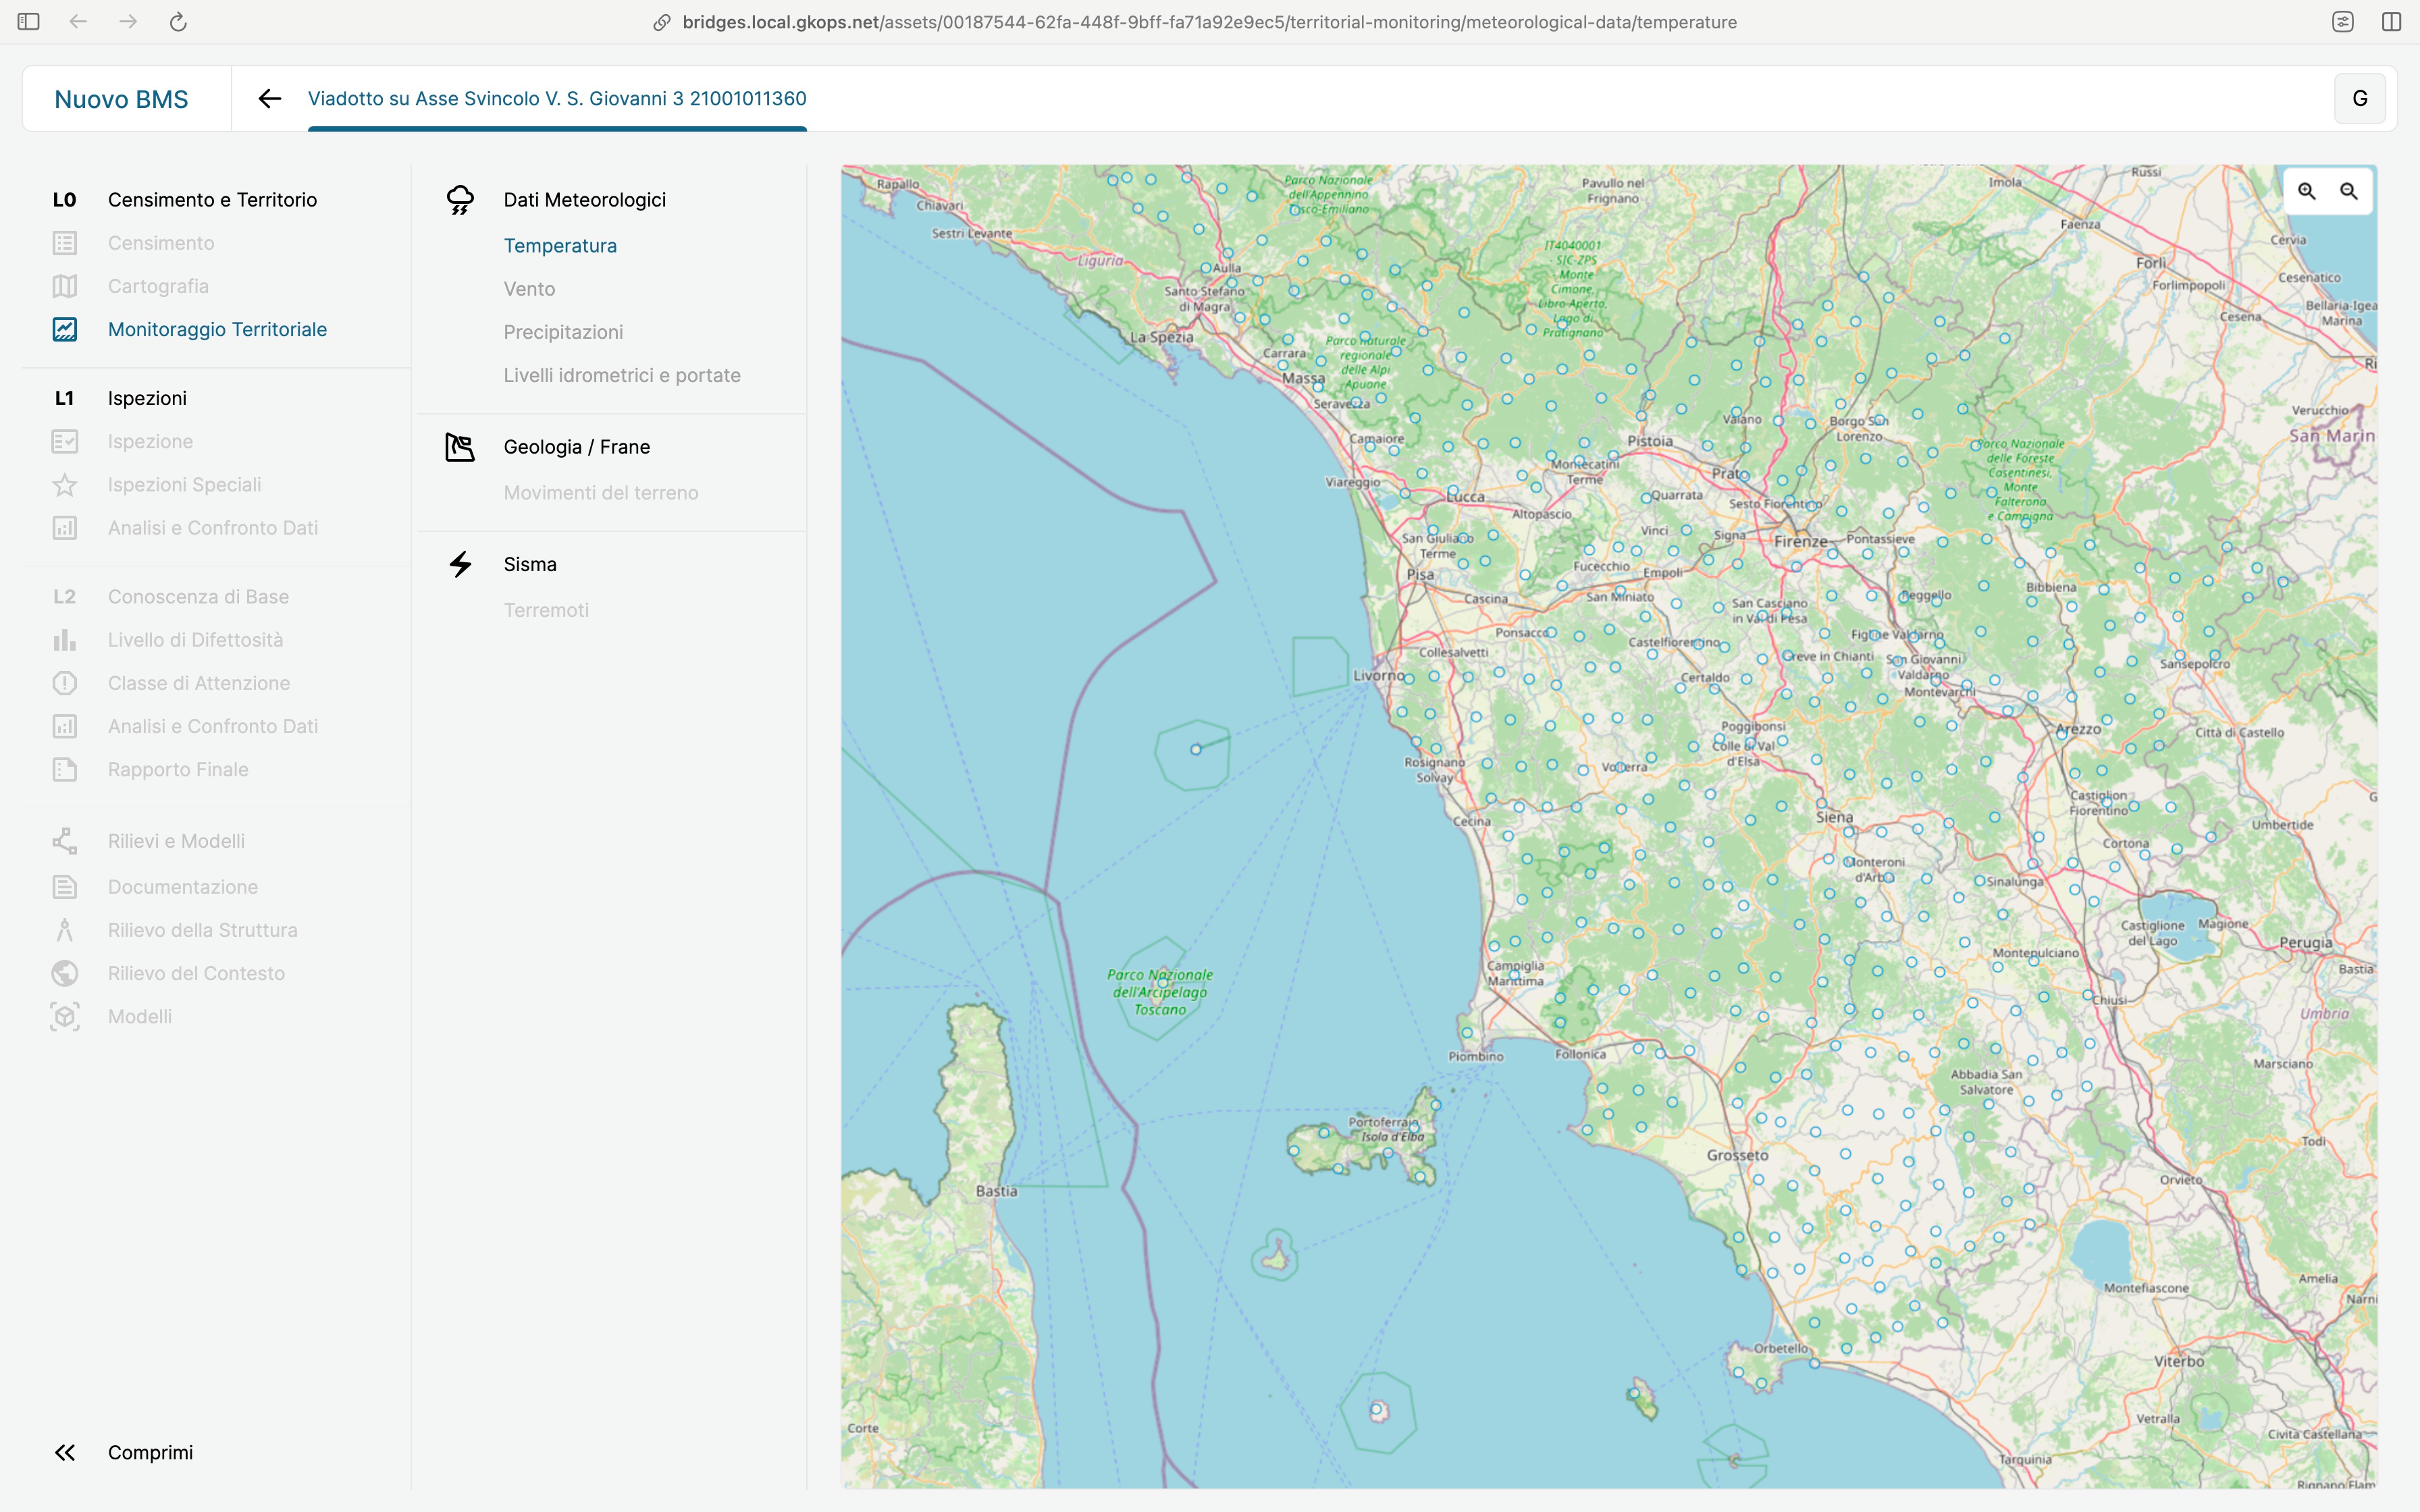
\includegraphics[width=1\textwidth]{Tesi/images/Capitolo4/toscanaGeoJSON.jpg}
      \caption{Mappa delle frane in Toscana, formato GeoJSON}
      \label{fig:toscanaGeoJSON}
\end{figure}

\subsection{Risoluzione del problema di stile con i punti}

Tuttavia, come si può notare dall'immagine \ref{fig:toscanaGeoJSON}, i punti mostrati sulla mappa non erano molto visibili. Inoltre, risultava difficile comprendere se il punto che si stava osservando era un punto di cluster o meno e, nel caso fosse stato un punto di cluster, non era chiaro quanti punti contenesse al suo interno. 
\\Il tirocinante si è quindi occupato di applicare uno stile ai nuovi punti ottenuti, distinguendoli così da quelli appartenenti a "cluster" piuttosto che a "non cluster". Sono stati così realizzati, facendo uso della classe \verb|Style| fornita dalla libreria di OpenLayers, tre stili: il primo si occupa di stilare il punto del cluster, il quale, oltre a renderlo più evidente, include un numero rappresentante i punti contenuti al suo interno. Il secondo, invece, riguarda il singolo punto non cluster, che si mostra come un triangolo rosso, così da essere facilmente visibile rispetto agli altri. L'ultimo, infine, è uno stile che serve a gestire gli errori: viene utilizzato per rappresentare i punti in cui lo stile scelto non viene applicato all'interno della mappa. Per essere subito notato, viene raffigurato come un triangolo giallo con un punto esclamativo al suo interno. Infine, questi stili sono stati poi inseriti all'interno di una nuova classe, nota con il nome di \verb|feature-style.ts|, così da averli organizzati in modo appropriato. Si veda l'immagine \ref{fig:toscanaGeoJSONStyle} per un esempio.
\begin{figure}[htbp]
      \centering
      \includegraphics[width=1\textwidth]{Tesi/images/Capitolo4/toscanaGeoJSONStyle.jpeg}
      \caption{Mappa delle frane in Toscana con stile applicato}
      \label{fig:toscanaGeoJSONStyle}
\end{figure}

\subsection{Risoluzione del problema di interazione con i punti}

L'ultimo problema che rimaneva da risolvere era quello di avere un meccanismo che potesse recuperare le informazioni di ogni singola Feature. A tale scopo, il tirocinante ha deciso di aggiungere la possibilità di poter cliccare su ogni punto mostrato sulla mappa. Nel dettaglio, si è fatto in modo che, al click di un utente su un punto, venisse mostrata una finestra, sempre in primo piano rispetto alla mappa sottostante, contenente le informazioni relative al punto selezionato.
\\Per fare ciò, è stato sufficiente registrare una nuova funzione sull'evento di click della Feature. Questa funzione si occupa di recuperare l'ID del punto cliccato e, successivamente, di individuare all'interno della lista di feature quella con l'ID corrispondente a quella appena ottenuta. Una volta recuperata, basta leggere il contenuto del campo "properties" al suo interno e mostrarlo a schermo nella finestra creata.
\\Tuttavia, i punti, essendo alcuni di loro dei cluster, non contengono direttamente al loro interno le informazioni della frana, peranto è stato necessario distinguere nuovamente un punto di "cluster" da uno "non cluster". Per fare ciò, è stato necessario aggiungere un controllo che si attiva quando l'utente clicca su un punto: se questo contiene al suo interno più elementi, allora si tratta di un cluster, mostrando nella finestra il numero di punti che contiene al suo interno. Altrimenti, se il punto interessato contiene un solo elemento, allora si tratta di una frana.
\\Il tirocinante ha infine implementato due diverse modalità di gestione del click: una in cui la schermata rimane aperta e si chiude solo se si clicca su un altro punto e l'altra che consente di avere più finestre aperte cliccando sui vari punti, permettendo così di confrontarli tra loro. Si veda l'immagine \ref{fig:toscanaClickGeoJSON} per un esempio.
\begin{figure}[htbp]
      \centering
      \includegraphics[width=1\textwidth]{Tesi/images/Capitolo4/toscanaClickGeoJSON.jpeg}
      \caption{Mappa delle frane in Toscana, informazioni della frana a schermo}
      \label{fig:toscanaClickGeoJSON}
\end{figure}

\subsection{Considerazioni sul risultato ottenuto}

Sebbene la mappa risultasse funzionante, in questo tipo di implementazione persistevano comunque dei problemi che non potevano essere trascurati. Il primo risiedeva nel fatto che, in quel momento, il file JSON della mappa era incluso direttamente all'interno del progetto; questo approccio potrebbe essere accettabile per scopi di debug o test, ma non poteva essere mantenuto in modo permanente: caricare centinaia di mappe direttamente nel front-end è inefficiente e sopratutto difficile da gestire. 
\\Un altro problema era che, fino ad allora, non era stato sviluppato alcun meccanismo che si occupasse di gestire l'inserimento di mappe in maniera dinamica. Infatti, la mappa era stata inserita in maniera "hard coded",  cioè nel codice era specificato esplicitamente quale mappa utilizzare, non permettendo quindi di supportare eventuali nuove mappe.
\\Inoltre, questa pratica consumava molte risorse, dato che il calcolo dei punti e delle proiezioni veniva eseguito direttamente dal front-end. Sarebbe quindi opportuno creare una figura, lato back-end, che si occupi dove possibile di eseguire direttamente il cambio di proiezione e fornire i dati calcolati al client. 
\\Infine, risultava difficile sviluppare un sistema che permettesse di limitare o manipolare la quantità di punti da caricare, in quanto il front-end era obbligato a leggere l'intero file JSON per eseguire questo tipo di operazioni.

\section{Integrazione del protocollo WMS}

Il tirocinante ha poi proseguito con l'implementazione del supporto al protocollo WMS. Tale protocollo è stato scelto come primo da integrare, in quanto è stato ritenuto dal candidato il più agevole rispetto agli altri standard. Questo è da ricercarsi nel fatto che il protocollo WMS, restituendo direttamente l'immagine di una mappa, non richiede di dover gestire la complessità delle tiles (come nel WMTS) o di dover rappresentare graficamente i dati ricevuti (come nel WFS).
\\Tuttavia, al contrario dell'implementazione precedente, non c'era più la possibilità di scaricare i dati di una mappa localmente ed inserirli all'interno del progetto, ma era obbligatorio reperire le immagini della mappa da un server esterno. Per fare ciò, quindi, era necessario realizzare un meccanismo che fosse in grado di effettuare una serie di richieste HTTP ad un server WMS, così da ricevere l'intera immagine della mappa e successivamente mostrarla a schermo nella giusta proiezione. Il tirocinante ha scelto, come prima mappa da integrare, la "Carta ecopedologica d'Italia" (figura \ref{fig:italiaWMS}), fornita da un server esterno del Geoportale Nazionale.
\\Il lavoro è quindi cominciato modificando ulteriormente le classi \verb|BuildLayer.ts| e \verb|MapModel.ts|, aggiungendo il supporto al protocollo WMS mediante l'uso della libreria di OpenLayers. Precisamente, si è fatto uso delle delle classi \verb|ImageWMS| e \verb|WMSCapabilities|, in quanto, come già spiegato, consentivano di eseguire le richieste HTTP al server WMS, senza doversi preoccupare di farle manualmente o di analizzare il contenuto delle loro risposte.
\\Il codice così scritto iniziava con una richiesta di GetCapabilities fatta al server del Geoportale Nazionale. Dopo aver ottenuto una risposta, veniva eseguito un parser, utilizzando la classe \verb|WMSCapabilities|, così da ottenere la lista di tutti i layer disponili con le rispettive proiezioni. Come risposta, il server forniva due layer accessibili: il primo, denominato "Carta ecopedologica - Generale" e il secondo "Carta ecopedologica - Dettaglio", entrambi disponibili in molte proiezioni, tra cui quella utilizzata da OpenLayers. Ciò ha implicato che, a differenza della mappa in GeoJSON precedentemente implementata, non era necessario eseguire il calcolo per effettuare il cambio di proiezione con Proj4.
\\Dopo aver scelto come primo layer da visualizzare "Carta ecopedologica - Generale", è stato sufficiente utilizzare la classe \verb|ImageWMS| che, passando il layer come parametro, ha eseguito automaticamente la richiesta GetMap al server, senza doversi preoccupare di inserire manualmente i query params corretti (come CRS, BBOX, FORMAT, etc...) per ricevere l'immagine della mappa.
\\Il lavoro del candidato è poi continuato aggiungendo alla sezione precedentemente sviluppata la nuova mappa disponibile, potendo così verificare se il codice da lui scritto fosse funzionante o meno.

\subsection{Caricamenti lenti e Rate Limiting}

La prima problematica riscontrata riguardava la lentezza delle risposte HTTP inviate dal server WMS per ottenere le immagini, causando notevoli ritardi nel caricamento della mappa selezionata.
\\Questo problema dipendeva sia dalla lentezza intrinseca dei loro server, sia dalla dimensione dell'immagine richiesta: essendo inviata tramite protocollo WMS, l'immagine non veniva divisa in tiles come in altri protocolli, ma veniva trasmessa attraverso una singola richiesta HTTP con l'intera immagine al suo interno, rendendo quindi più pesante il carico di ogni richiesta. In aggiunta, ogni volta che la telecamera veniva spostata, si effettuava nuovamente una richiesta al server per ricevere la nuova immagine, anche se questa poteva includere porzioni di mappa già presenti nella richiesta precedente.
\\Inoltre, dopo una serie di tentativi e varie richieste HTTP inviate allo stesso servizio, il server WMS del GeoPortale Nazionale ha iniziato a effettuare rate-limiting, cioè ha limitato il numero di richieste che potevano essere inviate in un determinato periodo di tempo, rendendo quindi la mappa non più accessibile.
\\Per ottenere comunque un risultato, è stato necessario limitare il più possibile il numero di richieste da inviare, evitando quindi di spostare troppo la telecamera della mappa per non generarne di nuove. 

\subsection{Considerazioni sul risultato ottenuto}

Sebbene la mappa venisse visualizzata correttamente e nella giusta proiezione, questo tipo di implementazione non era sostenibile a causa dei caricamenti lenti e del rate-limiting imposto dal server. 
\\Inoltre, similmente alla mappa in formato GeoJSON, il codice realizzato era progettato per funzionare esclusivamente con i suoi due rispettivi layer, senza possedere una struttura predisposta a supportare dinamicamente l'aggiunta di mappe ulteriori. In aggiunta, poiché la mappa veniva fornita con la stessa proiezione scelta da OpenLayers, non era stato implementato un sistema per gestire il cambio di proiezione come fatto precedentemente. Ciò poteva risultare un problema nel caso in cui altre mappe venissero fornite con una proiezione diversa, rendendo quindi necessaria un'adeguata gestione delle proiezioni per garantire la loro corretta visualizzazione.
\\Infine, tale sistema non garantiva l'affidabilità del servizio: se la mappa ospitata dai server veniva spostata, eliminata o se il server stesso diventava inattivo o soggetto a manutenzione, l'accesso alla mappa mediante l'applicazione veniva compromesso.
\\Quindi anche in questo caso, era necessario creare una figura esterna, situata all'interno del back-end, che si occupasse di risolvere principalmente queste complicazioni. 
\begin{figure}[htbp]
      \centering
      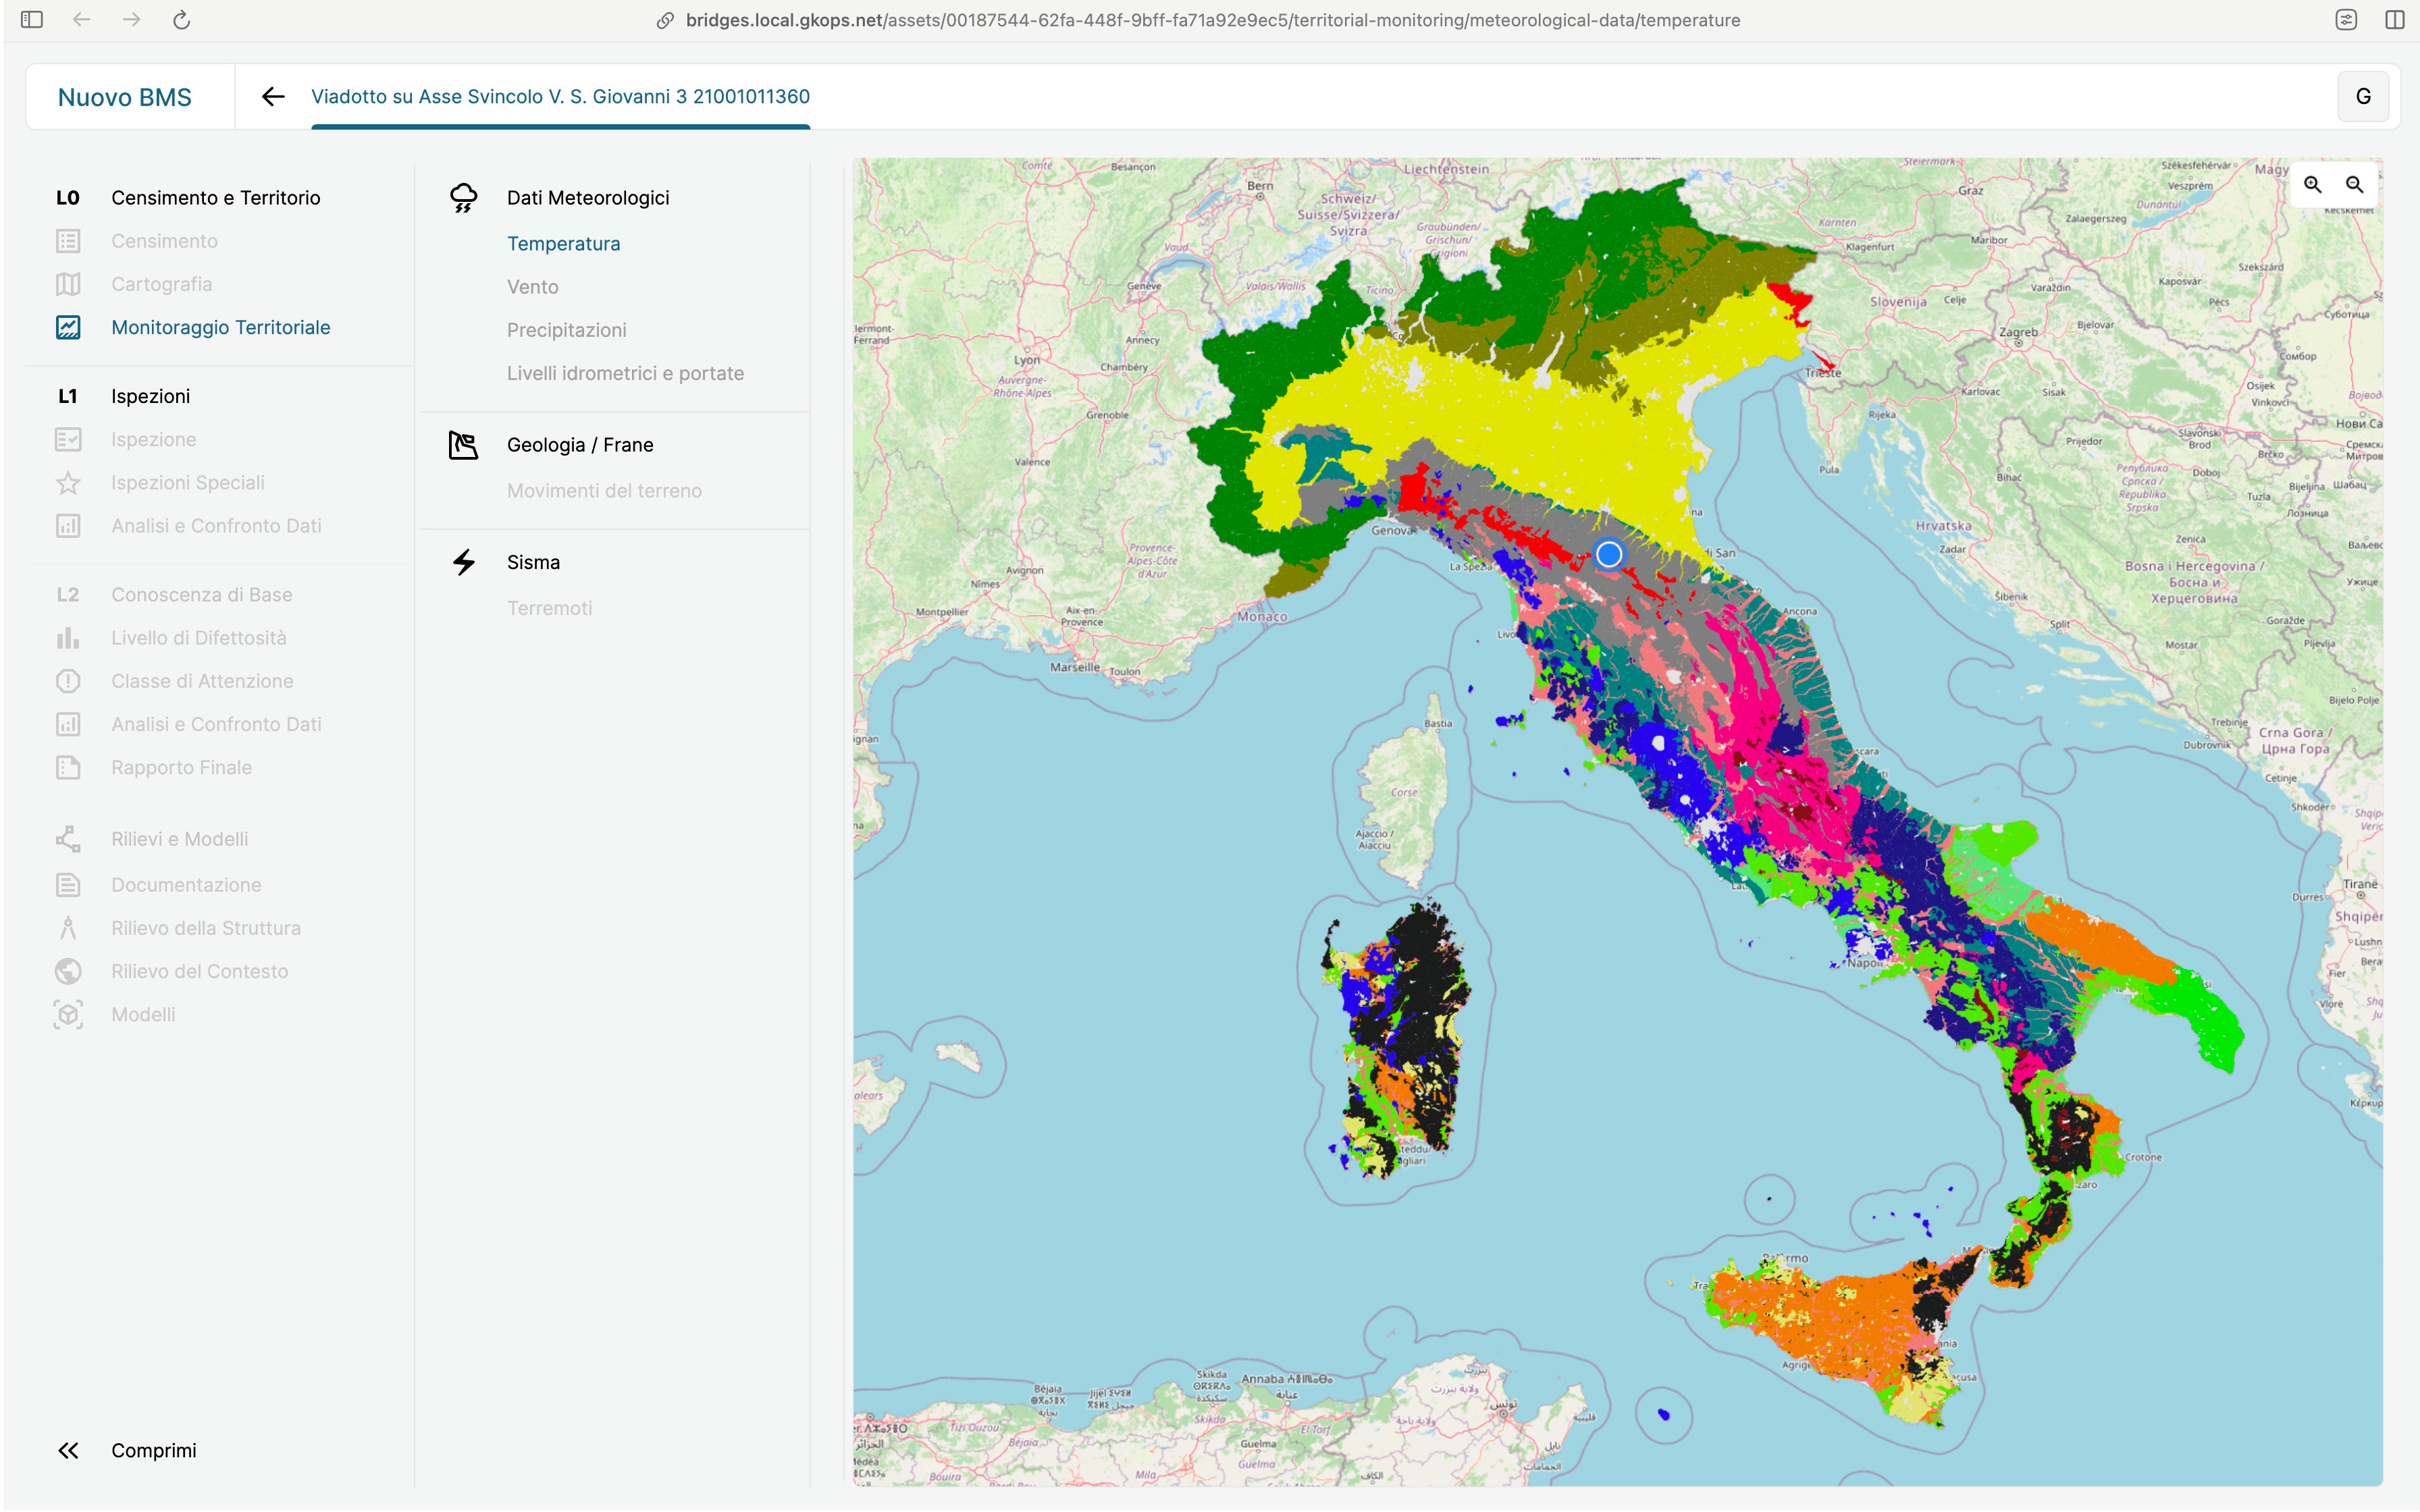
\includegraphics[width=1\textwidth]{Tesi/images/Capitolo4/italiaWMS.jpg}
      \caption{Carta ecopedologica - Generale, protocollo WMS}
      \label{fig:italiaWMS}
\end{figure}

%\lstinputlisting[language=Java, caption={Implementazione BuildLayer}]{listings/Capitolo4/buildLayer.js}